\section{Programming the PEs}
\label{chap:design}
In this chapter we discuss the requirements and the design for our automated programming of functional units, as well as the assembly language. Specifically, we go over the requirements the methodology needs to meet in \ref{sec:requirements}, we discuss the way the assembly has been defined in \ref{sec:assembly}, and we provide an overview of the methodology in \ref{sec:overview}, where we go over the individual parts of the methodology separately. %NOTE: Maybe not interesting to discuss implementation?

\section{Requirements}
\label{sec:requirements}
The output of the methodology is a list of FU instructions, discussed in \ref{sec:templates}, for every component in the architecture, such that the components behave as described by their respective FUs in the annotated DFG.

To guarantee the correctness of the execution according to the input application, the main requirement is that, for every operation in the annotated DFG, the component needs to be programmed to let the correct two inputs flow through the OP component at the time specified in the annotation of the operation.
To achieve this we define three more requirements which relate to the source for the input data for the OP component and the timing of the arrival of that input data.
% For this requirement we define three sub-requirements relating to the input data for the OP component and the timing of the arrival of the data.
First, we note that input can arrive on the input ports from other components, as described in \ref{sec:templates}. Thus, to be able to correctly read input data, we need to know which component is connected to which input port.
Second, we note that input data might arrive earlier than the operation on this data is scheduled to occur in the annotated DFG. Thus, we need to be able to temporarily store data that cannot be processed right away.
Third, and last, we need to fetch the data when the component is ready to perform the corresponding operation.

To allow us to design a methodology that meets these requirements we create an abstraction of the complex FU instructions. This abstraction is created by defining a high-level assembly language consisting of assembly instructions that each determine a subset of the fields of the FU instruction described in \ref{sec:templates}. We co-design the high-level assembly with the methodology such that each part of the methodology that meets one of these requirements will have a separate corresponding assembly instruction that it generates.

After the assembly instructions have been generated, they need to be compiled into FU instructions. To compile the assembly instructions we first need to merge them into full FU instructions, in which all fields are defined. We do this because the assembly instructions separately only determine subsets of the fields of an FU instruction. Next, because the sizes of the fields in the FU instructions differ per component, the fields of these FU instructions need to take up the correct number of bits such that they correspond with how the component is configured. Lastly, the sequence of FU instructions all need to be loaded into the IM of the component by generating the control signals as described in \ref{sec:templates} for each of them.

% \begin{itemize}
    % \item Generate op instructions for each node in cluster
    % \item Map the input ports of an FU to other FUs connected to it
    % \item Generate store and fetch instructions to store intermediate results
    % \item Generate control signals to facilitate loading of instructions and starting computation
    % \item ATA needs to be defined such that the problem can be more easily broken up into multiple pieces
    % \item Merge the ATAI
    % \item Format bitstrings to have correct length
% \end{itemize}

\section{Architecture Template Assembly specification}
\label{sec:assembly}
\begin{table}
    \centering
    \begin{tabular}{@{}l|ll@{}}
        \toprule
        input name & fields & description\\
        \hline
        OpInput & - & Input from the result of a previous $Op$ instruction\\
        FUInput & port & Input from one of the FU input ports\\
        RFInput & - & Input from the register file in the component\\
        \bottomrule
    \end{tabular}
    \caption{The input types which function as an abstraction to control the multiplexers, as well as which register in the RF data, coming from the input ports or as a result from a previously executed $Op$ instruction, is written to.}
    \label{tab:inputs}
\end{table}

\begin{table}
    \centering
    \begin{tabular}{@{}l|l p{.4\textwidth}@{}}
        \toprule
        instruction name & fields & description\\
        \hline
        Op & clock, input$_1$, input$_2$ & loads \$input$_1$ and \$input$_2$ into the OP part of the component at clock cycle \$clock. This input may or may not have a \$port value associated with it\\
        Fetch & clock, address, mux & Loads the bits from the RF at \$address and sends them to multiplexer \$mux at clock cycle \$clock\\
        Store & clock, input, address & Stores the bits from \$input in \$address at clock cycle \$clock\\
\bottomrule
    \end{tabular}
    \caption{All instructions in the Architecture Template Assembly we specified.}
    \label{tab:insts}
\end{table}
The Architecture Template Assembly (ATA) is designed to be an abstraction of the FU instruction discussed in \ref{sec:templates}. It is split into three different Architecture Template Assembly Instructions (ATAIs): $Op$, $Fetch$ and $Store$. Because all the instructions are executed at a specific, predetermined, clock cycle we define our ATA to always have a \$clock field. %NOTE: This is not a coherent introduction to the section, more of a collection of random sentences

To control the OP of the component, discussed in \ref{sec:templates}, we created the $Op$ instruction. This instruction focuses on the main requirement of letting two input flow through the OP part at the right time. It takes two input sources whose values are defined in \ref{tab:inputs}. $FUInput$ means that the data comes directly from the output of a different component through one of the input ports described in \ref{sec:templates}, thus it needs to have the field \$port to denote which of the ports should be read from. $OpInput$ means that the result of the previous computation of the component is used as input for the next. $RFInput$ means that the input comes from the RF, this only sets the multiplexer for the input described in \ref{sec:templates}. The actual fetching of the data from the RF happens through the $Fetch$ instruction.

The $Fetch$ instruction takes an RF address, which specifies the location where the data to fetch is located, as well as a multiplexer to send the data to.

The $Store$ instruction is used to store data in the RF. This instruction takes an input source as defined in \ref{tab:insts}. The values this field can have are the $FUInput$ and the $OpInput$ entries in \ref{tab:inputs}.

\newcommand{\rowgroup}[1]{\hspace{-0.5em}#1}
\begin{table}
    \centering
    \begin{tabular}{lll@{}}
        \toprule
        ATA field &  \multicolumn{2}{c}{MI fields}\\
        \hline
        clock & clock\\
        \rowgroup{$Op$}\\
        input$_1$ & muxA & cbOut0\\
        input$_2$ & muxB & cbOut1\\
        \rowgroup{$Fetch$ : mux=$x$}\\
        address & r\_REG$x$\_s\\
        \rowgroup{$Store$}\\
        address & w\_REG$x$\_s\\
        input & REG0 REG1 & cbOut2\\
        \bottomrule
    \end{tabular}
    \caption{Relation of the fields in the ATA instructions to the fields in the FU instructions.}
    \label{tab:ATA-MC}
\end{table}

\begin{table}
    \centering
    \begin{tabular}{@{}lll@{}}
        \toprule
        Input & Multiplexer value & cbOut value\\
        \hline
        OpInput & 0 & 0\\
        FUInput & 1 & port\\
        RFInput & 2 & 0\\
        \bottomrule
    \end{tabular}
    \caption{Values for the multiplexers and their correspondig cbOut ports depending the value of one of the `input' fields of the $Op$ instruction.}
    \label{tab:mux}
\end{table}

\begin{table}
    \centering
    \begin{tabular}{@{}llll@{}}
        \toprule
        Input & REG0 & REG1 & cbOut value\\
        \hline
        FUInput & - & 1 & port\\
        OpInput & 1 & - & 0\\
        \bottomrule
    \end{tabular}
    \caption{Values for REG0, REG1 and cbOut depending on the value of `input' of the $Store$ instruction.}
    \label{tab:reg}
\end{table}

The different ATA instruction types listen in \ref{tab:ATA-MC} are designed to never have any overlap in the fields they influence in the FU instruction. $Op$ determines the muxA, muxB, cbOut0 and cbOut1 fields depending on the values of the \$input$_1$ and \$input$_2$ fields as described in \ref{tab:mux}. $Fetch$ determines r\_REG0\_s or r\_REG1\_s. $Store$ determines w\_REG0\_s or w\_REG1\_s and their corresponding write-enable bits REG0 and REG1 as well as cbOut depending on the value of the \$input field as described in \ref{tab:reg}.`

% \begin{itemize}
    % \item All have a \$clock field
    % \item Op for data processing
    % \item Store and Fetch for interacting with the RF
    % \item Input types to determine where to source data from
    % \item High-level representation of the FU instructions
% \end{itemize}

\section{Methodology overview}
\label{sec:overview}

\begin{figure}
    \centering
    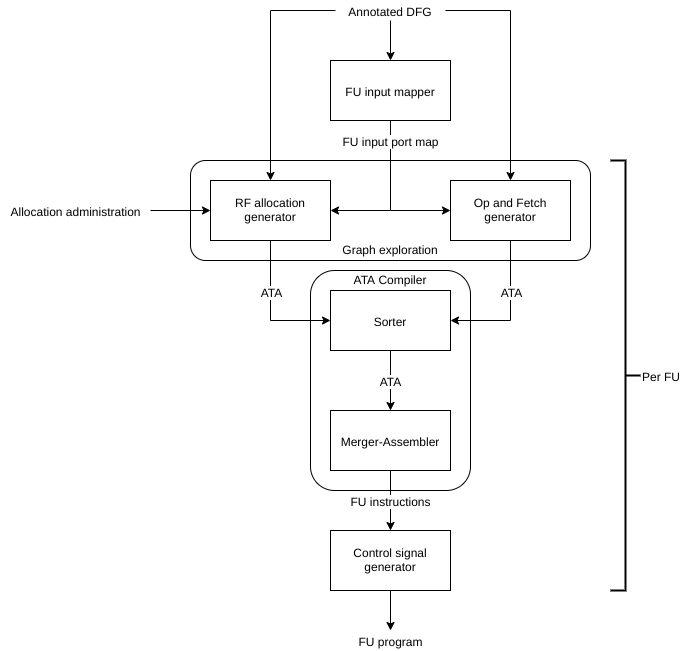
\includegraphics[scale=0.45]{graphs/methodology.png}
    \caption{Overview of the methodology (read from top to bottom).}
    \label{fig:framework}
\end{figure}

To meet the requirements laid out in \ref{sec:requirements}, we designed a methodology that takes as input an annotated DFG and an \textit{Allocation administration}, and produces a series of FU programs with some VHDL boilerplate code so they can be loaded into the IM of a component.

An overview of our methodology can be seen in \ref{fig:framework}. The methodology first analyses the interconnections between the FUs in the \textit{FU input mapper}, then looks at each FU in the annotated DFG separately. Next is the graph exploration phase, in which the FU in the annotated DFG is transformed into ATA instructions.
The \textit{RF allocation generator} generates the $Store$ instructions using both the annotated DFG and the \textit{Allocation administration} as inputs.
The \textit{Op and Fetch generator} then generates the $Op$ instructions as well as any required $Fetch$ instructions.
Next, the compiler phase starts, in which the ATA instructions are eventually turned into a list of FU instructions.
The \textit{Sorter} then sorts all the ATA instructions the methodology generates in the graph exploration phase by clock cycle, such that the \textit{ATA merger-assembler} can merge the ones occurring at the same clock cycle into a single FU instruction. Finally, for every generated FU instruction, the \textit{Control signal generator} sets all the ports and signals, as well as and the VHDL boilerplate code needed for loading the instruction into the IM (as described in \ref{sec:templates}).

\subsection*{Allocation administration}
The allocation administration is an analysis that is performed by the \frameworkname framework and provides an input for the methodology. It traverses the graph and determines if the output of an operation should be stored in the RF of the component that receives the output. The allocation administration then uses a customised interval partitioning algorithm to optimise the amount of memory being used by overwriting the data in the RF if the data is no longer needed. The allocation administration generates a map for each FU that describes what its memory layout should be. This map describes, for each piece of data in the RF, at which address it should be stored at, and from which node the data comes.

\subsection*{FU input mapper}
The \textit{FU input mapper}'s job is to map, for every component, all its output ports to the input ports of other components. For every FU in the annotated DFG, the input mapper produces an alphabetically sorted list of FUs whose output port is connected to one of the input ports. The index of each FU in this list corresponds to the port number to which it is connected. The output of the FU input mapper consists of this list.

% \begin{itemize}
    % \item Looks at the foreign incoming connections in the graph and sorts them alphabetically, then outputs of which ports map to which FU templates.
% \end{itemize}

\subsection*{RF allocation generator}
This phase generates $Store$ instructions, to ensure the storage of incoming data that cannot be immediately processed. The \textit{RF allocation generator} does this by consulting the map generated by the \textit{Allocation administration} for the current FU. A $Store$ instruction is generated for every entry in the map. The \$address field is found by simply consulting the entry in the map. The \$clock field is found by first finding the operation for which the entry in the map was generated. The latency of the OP of the component, as described in \ref{sec:templates}, is then added to the clock cycle for which it was scheduled. The \$input field is determined by looking if the operation resides in a foreign FU or not. The \textit{RF allocation generator} outputs the $Store$ instructions as a list, for which no order is guaranteed.

% \begin{itemize}
    % \item The RF allocation generator looks at incoming data from other FUs and creates $store$ instructions if needed
    % \item The $store$ instructions are generated by looking at the clock cycle at which the instruction generating the incoming data occurs, then adding the known latency for that instruction to it.
    % \item It outputs a list of ATAIs, the order of the ATAIs in the list is not guaranteed.
% \end{itemize}

%TODO: expand this section


\subsection*{Op and Fetch generator}
%The Op and Fetch generator generates all the $Op$ instructions as well as the $Fetch$ instructions to load the input data from the RF for the $Ops$.
As the name indicates, this module generates all the $Op$ instructions, as well as the $Fetch$ instructions to load the $Op$ input data from the RF.
The \textit{Op and Fetch generator} takes as input the annotated DFG, and (1) finds the FU describing the current component, and (2) generates an $Op$ instruction for every operation in this FU.
%By looking at the vertices in the annotated DFG representing inputs of the operations and comparing it with the map generated by the \textit{allocation administration} it decides for each input of $Op$ if it was stored in the RF or not.
By looking at the annotated DFG vertices representing operations inputs, and comparing them against the map generated by the \textit{allocation administration}, the Op and Fetch generator determines, for every $Op$ input, whether it is stored in the RF or not.
If the input is not in the RF, we look if the input vertex is in a foreign FU; in this case, we consult the map that the \textit{FU input mapper} generates to find the port this foreign FU is connected to.
We then set the input field of the $Op$ to $FUInput$ with the \$port field corresponding to the one found in the map. If the vertex is not in a foreign FU, and it is not stored in the RF, we set it to $OpInput$; if it is stored in the RF, we set it to $RFInput$ and generate a $Fetch$ instruction.
For this $Fetch$ instruction we first determine the \$clock field by subtracting the known fetch latency from the the clock cycle at which the $Op$ is scheduled. Next, we consult the allocation map and set the \$address field to the address where the data is stored. Finally, we set the \$mux field to 0 if the $Fetch$ instruction was generated as input for muxA, or 1 if it was generated for muxB.

The Op and Fetch generator outputs a list containing $Op$ and possibly $Fetch$ instructions. For this list no order is guaranteed.
% \begin{itemize}
    % \item Takes as input the annotated DFG and the current FU cluster
    % \item Generates $op$ instructions and $fetch$ instructions as needed to fetch the data needed for the $op$ from the register file.
    % \item Outputs all the ATAIs as a list for which no order is guaranteed.
% \end{itemize}

\subsection*{Sorter and ATA merger-assembler}
The \textit{sorter} takes as input the lists of ATA instructions that the graph traversal phase generates. And outputs a single list of ATA instructions, all sorted by clock cycle from low to high. The \textit{merger-assembler} converts the ATA instructions into FU instructions, and merges FU instructions occurring at the same clock cycle into a single one.

As described in \ref{sec:templates}, within one clock cycle we can store up to two words, fetch up to two words, and perform one operation. As such, the merger is able to merge at most: one $Op$ instruction, one $Store$ instruction for data from another component, one $Store$ instruction for data coming from an earlier $Op$ within the component, and two $Fetch$ instructions. Because we may not always merge the maximum of one $Op$, two $Store$ and two $Fetch$ instructions, some fields in a FU instruction may not be defined by the assembly. These fields are simply set to 0, which means that the two write-enable bits $REG0$ and $REG1$ are set to 0 if the assembly does not specify a $Store$ instruction at that clock cycle. This ensures we do not unintentionally overwrite any data in the RF. The other unspecified fields do not influence the behaviour of the component, no matter what value they contain; however setting them to 0 provides a more complete definition of what the \textit{merger-assembler} does.

%TODO: talk about this maximum amount of assembly a FU instruction can contain somewhere else as well (possibly in the ATA definition?)

Additionally, the \textit{merger-assemble} keeps track of the highest clock cycle, the RF address, and the amount of input ports, so it can format the FU instructions such that all the fields take up the correct amount of bits by padding them with 0s where necessary.
% \begin{itemize}
    % \item Sorter keeps a sorted list of ATAIs per FU
    % \item Merger-assembler merges ATAIs where possible/needed and converts it to ATMC
% \end{itemize}

\subsection*{Control signal generator}
After all the ATA instructions have been converted to FU instructions, the FU instructions still need to be loaded into the IM. For this, the control signals described \ref{sec:templates} need to be set. To facilitate this operation, the \textit{Control signal generator} first sets the r\_LOAD\_INST signal to 1. %NOTE: does this have to happen for every instruction loaded in memory? Not so sure.
Then the control signal generator adds the VHDL syntax for writing the FU instruction to the r\_INPUT\_INST port for every FU instruction. Additionally, the generator increments the IM address pointer after writing each instruction by setting the r\_LOAD\_NEXT\_INST to 1. Lastly, the \textit{Control signal generator} keeps track of how many clock cycles the components take to
load their instructions into the IM, to make sure all components start counting clock cycles at the same time, and none is still busy loading instructions; this synchronisation is achieved by setting the r\_COMPUTING signal to 1. The \textit{control signal generator} outputs a string of VHDL code, which can be inserted into the template of every component in the network. %NOTE: The part about syncing the computation still needs to be implemented.
% \begin{itemize}
    % \item Generates control signals for the template to facilitate loading instructions and starting execution
% \end{itemize}


%%% Local Variables:
%%% mode: latex
%%% TeX-master: "../dsd20_main"
%%% End:
